% In this section you describe the knowledge that the reader needs to understand your work and your contribution. Present basic knowledge needed to understand the area and the task. For example, you can describe relevant theories here and explain concepts you use or introduce mathematical notation. Write the background so that anyone who is well versed in the area can skip it.

\section{Background}

This is the background to the report. This section should be organized with subsection for etch of the areas explained.

This section will have most and at lest some citations. With APA thre are two ways name (Year) and (name, year) this is done with ''\textbackslash textcite\{bibtex-refrence\}'' for name (Year) and ''\textbackslash parencite\{bibtex-refrence\}''. Doing page numbering of sources is done via [p. Page] before the curly bracket. Muliible cations in the same place is done as a comma seperated list within the curly brackets.




\subsection{Citation example}
Example, \textcite[p. 321]{ieeeSDN} wrote about SDN. SDN is a technology for centralizing networking planes via software \parencite[p. 123]{ieeeSDN, Roadto}. This communication can be seen in Figure \ref{figureRefenceName}.


\begin{figure}[h]
	\centering
	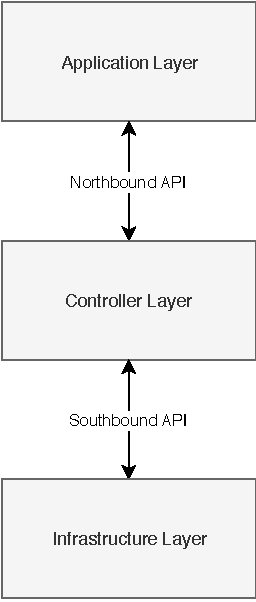
\includegraphics[width=0.25 \textwidth]{./pics/APIlayers.pdf}
	\caption{Figure caption}
    \label{figureRefenceName}
\end{figure}





